\documentclass[11pt,border=5pt]{standalone}
\usepackage{fontspec}
\setmainfont{cmunrm.otf}[BoldFont=cmunbx.otf,ItalicFont=cmunti.otf,BoldItalicFont=cmunbi.otf]
\usepackage{amsmath}
\usepackage{unicode-math}
\setmathfont{NewCMMath-Regular.otf}
\usepackage{tikz}
\usetikzlibrary{arrows.meta,patterns,angles,quotes}
\begin{document}
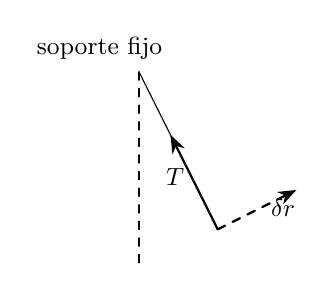
\begin{tikzpicture}[>=Stealth,font=\small,line cap=round,line join=round]
\draw[dashed] (0,1.5)--(0,-1);\draw (0,1.5)--(1,-.5);
\draw[->,thick,dashed] (1,-0.5) -- (2,-0.0) node[pos=0.55,right] {$\delta r$};
\draw[->,thick] (1,-0.5) -- (0.4,0.7) node[pos=0.55,left] {$T$};
\node at (-0.5,1.8) {soporte fijo};

\end{tikzpicture}
\end{document}
